\section{Theoretical Foundations of Classical Optimization Algorithms}

Traditional optimization methods not only form the fundamental principles of modern algorithms but also remain among the most reliable tools for solving engineering problems. In this section, we will provide an in-depth look at the mathematical foundations of these methods and examine how they are applied to structural optimization problems.

\subsection{Analytical Foundations of Mathematical Optimization}

Optimization has been one of the most fundamental problems throughout mathematical history. Even before Leibniz and Newton developed differential calculus, mathematicians were dealing with optimization problems. In the modern sense, the analytical foundations of mathematical optimization are based on three fundamental concepts: stationarity, convexity, and duality.

\begin{tcolorbox}[title=Historical Perspective]
\begin{itemize}
    \item \textbf{Ancient Greece:} Euclidean geometry and maximum-minimum problems
    \item \textbf{17th Century:} Fermat, Leibniz, and Newton's differential calculus
    \item \textbf{18th Century:} Lagrange and Euler's variational calculations
    \item \textbf{19th Century:} Hamilton and Jacobi's optimization theories
    \item \textbf{20th Century:} Development of linear programming, numerical optimization, and complex algorithms
\end{itemize}
\end{tcolorbox}

\subsubsection{First and Second Order Optimality Conditions}

The most important analytical conditions that form the mathematical basis of optimization are:

\textbf{First Order Necessary Condition (Stationarity):} 
If $x^*$ is a local minimum, then $\nabla f(x^*) = 0$ must hold. This means that the gradient of the function is zero, i.e., the tangent plane is horizontal.

\textbf{Second Order Sufficient Condition:} 
If $\nabla f(x^*) = 0$ and the Hessian matrix $\nabla^2 f(x^*)$ is positive definite, then $x^*$ is a strict local minimum. Mathematically, for all $d \neq 0$, the condition $d^T \nabla^2 f(x^*) d > 0$ must be satisfied.

\sidenote{Second order conditions help us determine whether a critical point (where the gradient is zero) is a local minimum, local maximum, or a saddle point. In structural optimization problems, the evaluation of the Hessian matrix is critical for the algorithm's progress.}

\subsubsection{Special Case of Convex Optimization}

Convex optimization is a special case of classical optimization theory and has remarkable properties:

\begin{itemize}
    \item If the objective function and constraint set are convex, every local minimum is also a global minimum
    \item In convex problems, critical point conditions guarantee the global optimum
    \item In structural mechanics, potential energy minimization for linear elastic structures is a convex problem
    \item Even for non-convex problems, they can often be decomposed into convex subproblems
\end{itemize}

\begin{marginfigure}
\centering
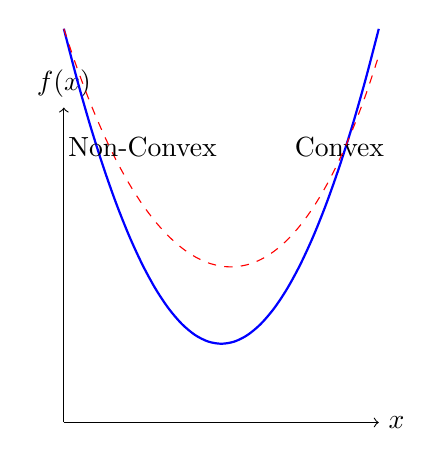
\begin{tikzpicture}
\draw[->] (0,0) -- (4,0) node[right] {$x$};
\draw[->] (0,0) -- (0,4) node[above] {$f(x)$};

% Convex and non-convex functions
\draw[scale=1,domain=0:4,smooth,variable=\x,blue,thick] plot ({\x},{(\x-2)^2+1});
\node at (3.5,3.5) {Convex};

\draw[scale=1,domain=0:4,smooth,variable=\x,red,dashed] plot ({\x},{sin(50*\x)+(\x-2)^2+1});
\node at (1,3.5) {Non-Convex};

\end{tikzpicture}
\caption{Comparison of convex and non-convex functions}
\label{fig:convexity}
\end{marginfigure}

\subsection{Gradient-Based Optimization Algorithms}

Gradient-based algorithms are methods that systematically approach the optimum point using derivative information of the function. These methods are of great importance in structural optimization problems in terms of computational efficiency and convergence properties.

\subsubsection{Gradient Descent Method and Its Variations}
The gradient descent method is the most basic and oldest gradient-based optimization method. This method aims to reach the minimum point by moving in the direction of the steepest descent of the function.

\begin{equation}
x_{k+1} = x_k - \alpha_k \nabla f(x_k)
\end{equation}

Here, $\alpha_k$ represents the step size (or learning rate) and significantly affects the algorithm's performance.

\begin{tcolorbox}[title=Gradient Descent Variations]
\begin{itemize}
    \item \textbf{Fixed Step Size:} The simplest approach uses a constant $\alpha$ for all iterations. However, it may be too low for fast convergence or too high for stability.
    
    \item \textbf{Line Search:} In each iteration, the value of $\alpha_k$ that minimizes $f(x_k - \alpha \nabla f(x_k))$ is found. This approach can be implemented with Armijo, Wolfe, or Goldstein conditions.
    
    \item \textbf{Momentum Gradient Descent:} Considers previous gradient values to reduce getting stuck in local minima:
    $$x_{k+1} = x_k - \alpha_k \nabla f(x_k) + \beta (x_k - x_{k-1})$$
    
    \item \textbf{Nesterov Accelerated Gradient:} An improved version of momentum gradient descent, it calculates the gradient not at the current position but at the point where momentum would take it.
\end{itemize}
\end{tcolorbox}

\sidenote{In structural optimization problems, the gradient descent method is typically used in the initial stages of large-scale problems. Although its convergence rate is low, its computational cost is low and it can provide a good starting point for complex problems.}

\begin{marginfigure}
\centering
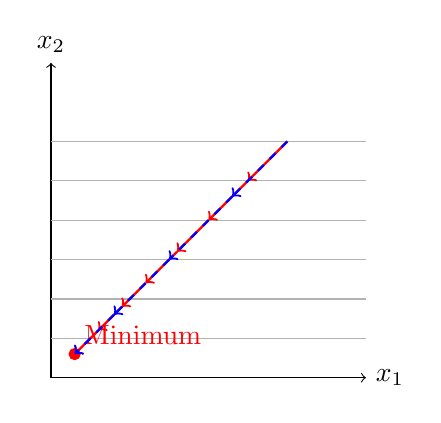
\begin{tikzpicture}
\draw[->] (0,0) -- (4,0) node[right] {$x_1$};
\draw[->] (0,0) -- (0,4) node[above] {$x_2$};

% Contour lines
\draw[scale=1,domain=0:4,smooth,variable=\x,black!30,thin] plot ({\x},{0.5});
\draw[scale=1,domain=0:4,smooth,variable=\x,black!30,thin] plot ({\x},{1.0});
\draw[scale=1,domain=0:4,smooth,variable=\x,black!30,thin] plot ({\x},{1.5});
\draw[scale=1,domain=0:4,smooth,variable=\x,black!30,thin] plot ({\x},{2.0});
\draw[scale=1,domain=0:4,smooth,variable=\x,black!30,thin] plot ({\x},{2.5});
\draw[scale=1,domain=0:4,smooth,variable=\x,black!30,thin] plot ({\x},{3.0});

% Gradient descent path
\draw[->,red,thick] (3,3) -- (2.5,2.5);
\draw[->,red,thick] (2.5,2.5) -- (2.0,2.0);
\draw[->,red,thick] (2.0,2.0) -- (1.6,1.6);
\draw[->,red,thick] (1.6,1.6) -- (1.2,1.2);
\draw[->,red,thick] (1.2,1.2) -- (0.9,0.9);
\draw[->,red,thick] (0.9,0.9) -- (0.6,0.6);
\draw[->,red,thick] (0.6,0.6) -- (0.3,0.3);
\filldraw[red] (0.3,0.3) circle (2pt) node[above right] {Minimum};

% Momentum gradient descent path
\draw[->,blue,thick,dashed] (3,3) -- (2.3,2.3);
\draw[->,blue,thick,dashed] (2.3,2.3) -- (1.5,1.5);
\draw[->,blue,thick,dashed] (1.5,1.5) -- (0.8,0.8);
\draw[->,blue,thick,dashed] (0.8,0.8) -- (0.3,0.3);

\end{tikzpicture}
\caption{Comparison of gradient descent (red, solid) and momentum gradient descent (blue, dashed) methods}
\label{fig:gradient_descent_variants}
\end{marginfigure}

\paragraph{Gradient Calculation in Structural Optimization}
In structural optimization problems, three methods are typically used for gradient calculation:

\begin{itemize}
    \item \textbf{Analytical Gradient:} Obtained through direct differential calculation. Provides the most accurate result but derivative derivation can be difficult in complex systems.
    
    \item \textbf{Finite Differences:} Gradient is calculated using numerical approximation:
    $$\frac{\partial f}{\partial x_i} \approx \frac{f(x + h e_i) - f(x)}{h}$$
    Easy to compute but the choice of $h$ is sensitive and computational cost is high for large systems.
    
    \item \textbf{Adjoint Method:} Particularly efficient for large-scale structural problems. Requires a constant number of system solutions independent of the number of design variables. Frequently used in finite element analysis.
\end{itemize}

\subsubsection{Newton and Quasi-Newton Methods}
The Newton method is one of the most powerful tools in classical optimization. It uses second-order derivative information (Hessian matrix) to create a local quadratic approximation of the function and moves directly toward the minimum point of this approximation.

\begin{equation}
x_{k+1} = x_k - [\nabla^2 f(x_k)]^{-1} \nabla f(x_k)
\end{equation}

The greatest advantage of the Newton method is its quadratic convergence rate; that is, as it approaches the optimum point, the error decreases approximately by the square in each iteration. However, calculating and inverting the Hessian matrix is computationally expensive, especially for high-dimensional problems.

\paragraph{Modified Newton Methods}
Various modifications have been developed to reduce computational cost and achieve better performance in cases where the Newton method might be unstable:

\begin{itemize}
    \item \textbf{Levenberg-Marquardt Algorithm:} Modifies the Hessian matrix to make it more stable:
    $$x_{k+1} = x_k - [\nabla^2 f(x_k) + \lambda I]^{-1} \nabla f(x_k)$$
    Here, $\lambda$ is a damping parameter that adjusts the algorithm's behavior.
    
    \item \textbf{Trust Region Newton Method:} Defines a "trust region" in each iteration where the Hessian matrix is valid and minimizes the quadratic model within this region. Particularly common in structural optimization.
\end{itemize}

\paragraph{Quasi-Newton Methods}
To eliminate the computational cost of calculating the full Hessian matrix, quasi-Newton methods iteratively update an approximation of the Hessian matrix. The most popular quasi-Newton methods are:

\begin{equation}
x_{k+1} = x_k - B_k^{-1} \nabla f(x_k)
\end{equation}

Here, $B_k$ is the approximation of the Hessian matrix at the $k$th iteration.

\begin{tcolorbox}[title=Basic Quasi-Newton Algorithms]
\begin{itemize}
    \item \textbf{BFGS (Broyden-Fletcher-Goldfarb-Shanno):} The most widely used quasi-Newton method. Maintains the positive definiteness of the Hessian approximation, which increases the algorithm's stability. Frequently preferred in structural optimization problems.
    
    \item \textbf{DFP (Davidon-Fletcher-Powell):} An older method than BFGS, but generally not as stable.
    
    \item \textbf{SR1 (Symmetric Rank-One):} Requires less computation but does not guarantee positive definiteness.
    
    \item \textbf{L-BFGS (Limited-memory BFGS):} A memory-optimized version of BFGS developed for very high-dimensional problems. Preferred in large-scale structural optimization problems, especially in topology optimization.
\end{itemize}
\end{tcolorbox}

\paragraph{Newton and Quasi-Newton Applications in Structural Optimization}
In structural engineering, Newton and quasi-Newton methods are frequently used in the following types of problems:

\begin{itemize}
    \item \textbf{Shape Optimization:} In optimizing the external geometry of structures, especially for aerodynamic performance or thermal behavior
    
    \item \textbf{Cross-Section Optimization:} In optimizing element cross-sections of truss and frame structures, especially in structures exhibiting nonlinear behavior
    
    \item \textbf{Parameter Calibration:} In calibrating finite element models with experimental data, determining material parameters
    
    \item \textbf{Multi-physics Optimization:} In complex engineering problems where structural, thermal, and fluid behaviors are optimized together
\end{itemize}

\begin{marginfigure}
\centering
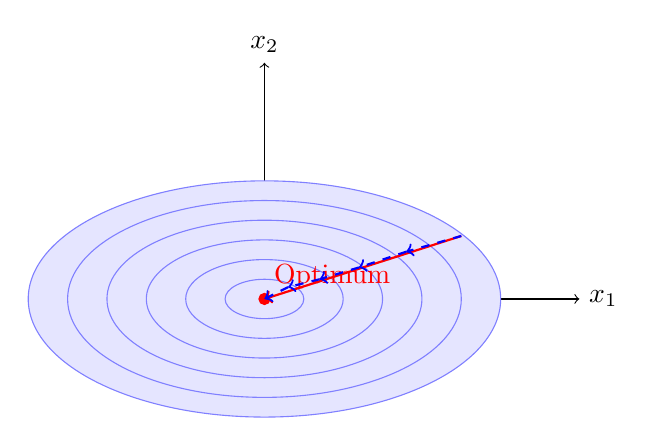
\begin{tikzpicture}
\draw[->] (0,0) -- (4,0) node[right] {$x_1$};
\draw[->] (0,0) -- (0,3) node[above] {$x_2$};

% Contour lines
\fill[blue!10] (0,0) ellipse (3 and 1.5);
\draw[blue!50] (0,0) ellipse (0.5 and 0.25);
\draw[blue!50] (0,0) ellipse (1 and 0.5);
\draw[blue!50] (0,0) ellipse (1.5 and 0.75);
\draw[blue!50] (0,0) ellipse (2 and 1);
\draw[blue!50] (0,0) ellipse (2.5 and 1.25);
\draw[blue!50] (0,0) ellipse (3 and 1.5);

% Newton path
\draw[->,red,thick] (2.5,0.8) -- (0,0);
\filldraw[red] (0,0) circle (2pt) node[above right] {Optimum};

% Gradient descent path
\draw[->,blue,thick,dashed] (2.5,0.8) -- (1.8,0.6);
\draw[->,blue,thick,dashed] (1.8,0.6) -- (1.2,0.4);
\draw[->,blue,thick,dashed] (1.2,0.4) -- (0.7,0.25);
\draw[->,blue,thick,dashed] (0.7,0.25) -- (0.3,0.15);
\draw[->,blue,thick,dashed] (0.3,0.15) -- (0,0);

\end{tikzpicture}
\caption{Comparison of Newton method (red, solid) and gradient descent method (blue, dashed). The Newton method can reach the optimum in a single step for quadratic functions.}
\label{fig:newton_vs_gradient}
\end{marginfigure}

\subsection{Constrained Optimization and Duality Theory}

Engineering problems rarely appear unconstrained. In structural design, there are many constraints such as stress limits, displacement boundaries, physical constraints, and resource limitations. In this section, we will examine in depth the classical approaches to solving constrained optimization problems.

\subsubsection{Lagrange Multipliers Method and Theoretical Foundations}

The Lagrange multipliers method is a fundamental approach developed for solving equality-constrained optimization problems. Developed by Joseph-Louis Lagrange in the 18th century, this method is one of the cornerstones of optimization theory and variational calculus.

An equality-constrained optimization problem is expressed as:
\begin{equation}
\begin{aligned}
\min & \quad f(x) \\
\text{s.t.} & \quad h_j(x) = 0, \quad j = 1, \ldots, p
\end{aligned}
\end{equation}

The Lagrange function (or Lagrangian) is defined as:
\begin{equation}
\mathcal{L}(x,\lambda) = f(x) + \sum_{j=1}^p \lambda_j h_j(x)
\end{equation}

Here, the $\lambda_j$ values are called Lagrange multipliers and represent the "shadow price" or marginal value of each constraint.

\sidenote{In structural engineering, Lagrange multipliers often have physical meaning. For example, in an optimization problem where we use force equilibrium as a constraint, the Lagrange multipliers typically correspond to displacements. This duality is a fundamental concept in finite element analysis and structural optimization.}

\paragraph{Lagrange Conditions}
The necessary conditions for a local minimum of a constrained optimization problem are:

\begin{equation}
\begin{aligned}
\nabla_x \mathcal{L}(x^*,\lambda^*) &= \nabla f(x^*) + \sum_{j=1}^p \lambda_j^* \nabla h_j(x^*) = 0 \\
\nabla_{\lambda} \mathcal{L}(x^*,\lambda^*) &= h_j(x^*) = 0, \quad j = 1, \ldots, p
\end{aligned}
\end{equation}

These conditions express that at the optimal point, the gradient of the objective function must be equal to a linear combination of the gradients of the constraint functions. Geometrically, this means that the level curves of $f(x)$ and $h_j(x)$ must be tangent.

\begin{figure}
\centering
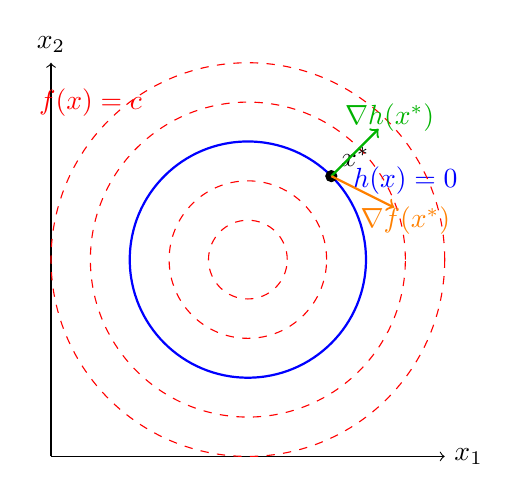
\begin{tikzpicture}
\draw[->] (0,0) -- (5,0) node[right] {$x_1$};
\draw[->] (0,0) -- (0,5) node[above] {$x_2$};

% Constraint function (a circle)
\draw[blue,thick] (2.5,2.5) circle (1.5);
\node[blue] at (4.5,3.5) {$h(x) = 0$};

% Objective function level curves
\draw[red,dashed] (2.5,2.5) circle (0.5);
\draw[red,dashed] (2.5,2.5) circle (1);
\draw[red,dashed] (2.5,2.5) circle (2);
\draw[red,dashed] (2.5,2.5) circle (2.5);
\node[red] at (0.5,4.5) {$f(x) = c$};

% Optimum point
\filldraw[black] (3.56,3.56) circle (2pt) node[above right] {$x^*$};

% Gradients
\draw[->,green!70!black,thick] (3.56,3.56) -- (4.16,4.16);
\node[green!70!black] at (4.3,4.3) {$\nabla h(x^*)$};

\draw[->,orange,thick] (3.56,3.56) -- (4.36,3.16);
\node[orange] at (4.5,3) {$\nabla f(x^*)$};

\end{tikzpicture}
\caption{Geometric interpretation of the Lagrange multipliers method: At the optimum point, the level curve of the objective function is tangent to the level curve of the constraint function.}
\label{fig:lagrange_geometry}
\end{figure}

\paragraph{Second Order Conditions}
To determine whether a critical point is actually a minimum, the extended Hessian matrix must be examined. If this matrix is positive definite in the tangent space of the constraints, the critical point is considered a local minimum.

\begin{tcolorbox}[title=Applications of Lagrange Method in Structural Optimization]
\begin{itemize}
    \item \textbf{Steel Frame Structures:} Ensuring force equilibrium at nodes and element compatibility while minimizing weight
    
    \item \textbf{Composite Material Design:} Ensuring volume constraint and material balance conditions while maximizing stiffness
    
    \item \textbf{Truss Systems:} Ensuring isostatic equilibrium conditions while minimizing weight
    
    \item \textbf{Finite Element Analysis:} Ensuring kinematic compatibility and force equilibrium constraints in finite element formulations based on energy minimization principle
\end{itemize}
\end{tcolorbox}

\subsubsection{Karush-Kuhn-Tucker (KKT) Conditions and Inequality Constraints}

The Karush-Kuhn-Tucker (KKT) conditions are a generalization of the Lagrange multipliers method for inequality-constrained problems. These conditions provide a fundamental framework for characterizing optimal solutions in the field of nonlinear programming.

An inequality-constrained optimization problem is expressed as:
\begin{equation}
\begin{aligned}
\min & \quad f(x) \\
\text{s.t.} & \quad g_i(x) \leq 0, \quad i = 1, \ldots, m \\
& \quad h_j(x) = 0, \quad j = 1, \ldots, p
\end{aligned}
\end{equation}

The Lagrange function in this case is:
\begin{equation}
\mathcal{L}(x,\lambda,\mu) = f(x) + \sum_{i=1}^m \mu_i g_i(x) + \sum_{j=1}^p \lambda_j h_j(x)
\end{equation}

\paragraph{KKT Conditions}
The necessary conditions for a local minimum of an inequality-constrained problem (KKT conditions) are:

\begin{equation}
\begin{aligned}
\nabla f(x^*) + \sum_{i=1}^m \mu_i^* \nabla g_i(x^*) + \sum_{j=1}^p \lambda_j^* \nabla h_j(x^*) &= 0 \\
g_i(x^*) &\leq 0, \quad i = 1, \ldots, m \\
h_j(x^*) &= 0, \quad j = 1, \ldots, p \\
\mu_i^* &\geq 0, \quad i = 1, \ldots, m \\
\mu_i^* g_i(x^*) &= 0, \quad i = 1, \ldots, m
\end{aligned}
\end{equation}

The last condition is known as "complementary slackness" and expresses that a constraint must either be active (satisfied as equality) or its corresponding Lagrange multiplier must be zero.

\begin{tcolorbox}[title=Interpretation of KKT Conditions]
\begin{itemize}
    \item \textbf{Stationarity:} The gradient of the objective function must be expressed as a linear combination of the gradients of active constraints. This shows that at the optimum point, progress is not possible without violating at least one active constraint.
    
    \item \textbf{Primal Feasibility:} All constraints must be satisfied.
    
    \item \textbf{Dual Feasibility:} The Lagrange multipliers (Kuhn-Tucker multipliers) for inequality constraints must be non-negative. This shows that the direction of constraints is important.
    
    \item \textbf{Complementary Slackness:} If any constraint is not active (satisfied as inequality), its corresponding Lagrange multiplier must be zero. This means the constraint is "inactive."
\end{itemize}
\end{tcolorbox}

\paragraph{Importance of KKT Conditions in Structural Optimization}
Structural optimization problems typically involve numerous inequality constraints. For example:
\begin{itemize}
    \item Stress constraints: $\sigma_i \leq \sigma_{allow}$
    \item Displacement constraints: $|u_i| \leq u_{allow}$
    \item Buckling constraints: $P_i \leq P_{cr,i}$
    \item Geometric constraints: minimum thickness, width, etc.
\end{itemize}

In such problems, KKT conditions provide not only a mathematical tool but also a framework with physical meaning. For example, the Lagrange multiplier associated with a stress constraint shows the effect of a unit stress increase at the relevant point on the weight of the optimal design. This is a fundamental concept for "design sensitivity analysis."

\begin{marginfigure}
\centering
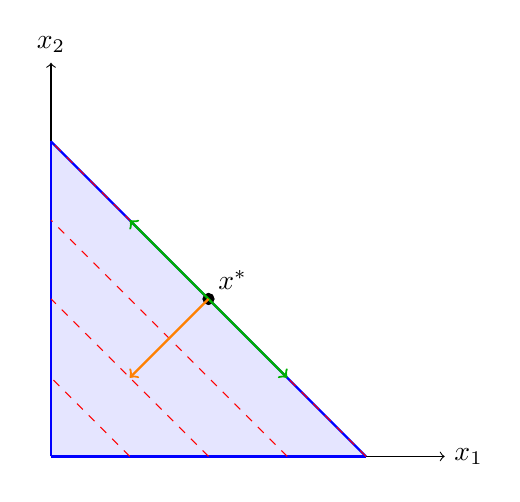
\begin{tikzpicture}
\draw[->] (0,0) -- (5,0) node[right] {$x_1$};
\draw[->] (0,0) -- (0,5) node[above] {$x_2$};

% Feasible region
\fill[blue!10] (0,0) -- (0,4) -- (2,2) -- (4,0) -- cycle;
\draw[blue,thick] (0,4) -- (2,2) -- (4,0);
\draw[blue,thick] (0,0) -- (0,4);
\draw[blue,thick] (0,0) -- (4,0);

% Objective function level lines
\draw[red,dashed] (1,0) -- (0,1);
\draw[red,dashed] (2,0) -- (0,2);
\draw[red,dashed] (3,0) -- (0,3);
\draw[red,dashed] (4,0) -- (0,4);

% Optimum point
\filldraw[black] (2,2) circle (2pt) node[above right] {$x^*$};

% Gradients of active constraints
\draw[->,green!70!black,thick] (2,2) -- (3,1);
\draw[->,green!70!black,thick] (2,2) -- (1,3);

% Objective function gradient
\draw[->,orange,thick] (2,2) -- (1,1);

\end{tikzpicture}
\caption{Geometric interpretation of KKT conditions: At the optimum point, the negative gradient of the objective function lies in the convex cone of the gradients of active constraints.}
\label{fig:kkt_geometry}
\end{marginfigure}

\paragraph{Duality Theory and Economic Interpretation}
Lagrange duality examines the relationship between the primal problem and its dual problem. The dual problem involves maximizing the Lagrange function instead of minimizing it:

\begin{equation}
\begin{aligned}
\max_{\mu \geq 0, \lambda} \min_{x} \mathcal{L}(x,\lambda,\mu)
\end{aligned}
\end{equation}

The duality theorem states that for a convex primal problem, the optimal value of the dual problem equals the optimal value of the primal problem (strong duality). This theorem forms the basis of many optimization algorithms.

From an economic perspective, dual variables (Lagrange multipliers) represent "shadow prices." In structural optimization, this shows the effect of a marginal change in a constraint on the value of the optimal design. This interpretation allows engineers to understand which constraints have the greatest impact on the design.

\begin{tcolorbox}[title=Relationship Between Duality and Structural Analysis]
In structural mechanics, the relationship between potential energy minimization (displacement method) and complementary energy minimization (force method) is a perfect example of the duality concept in optimization theory.

For the analysis of a structure:
\begin{itemize}
    \item \textbf{Primal Problem (Displacement Method):} Minimizing potential energy to find the compatible displacement field
    \item \textbf{Dual Problem (Force Method):} Minimizing complementary energy to find the force distribution in equilibrium
\end{itemize}

This duality is also used in the design of structural optimization algorithms. Particularly, "primal-dual" methods solve both the primal and dual problems simultaneously, providing more efficient optimization.
\end{tcolorbox}

\subsection{Linear and Quadratic Programming}

An important subset of classical optimization methods consists of linear and quadratic programming methods. These methods provide efficient solution algorithms specifically developed for optimization problems with certain structures.

\subsubsection{Linear Programming and Structural Applications}

Linear programming (LP) examines optimization problems where both the objective function and constraints are linear. Standard form:

\begin{equation}
\begin{aligned}
\min & \quad c^T x \\
\text{s.t.} & \quad Ax = b \\
& \quad x \geq 0
\end{aligned}
\end{equation}

Linear programming made significant progress in the 1940s with George Dantzig's development of the Simplex algorithm. Today, Interior Point Methods are also widely used for large-scale linear programming problems.

\paragraph{Simplex Method and Geometric Interpretation}
The Simplex method aims to find the optimal solution by systematically examining the corner points (extreme points) of the feasible region. The fundamental theorem of LP states that the optimal solution must be at a corner point of the feasible region (if the solution is not unique).

The steps of this method:
\begin{itemize}
    \item Find a feasible corner point for initialization
    \item Move to a neighboring corner point that improves the objective function value
    \item Continue until no better neighboring corner point can be found
\end{itemize}

\begin{tcolorbox}[title=LP Applications in Structural Engineering]
\begin{itemize}
    \item \textbf{Plastic Limit Analysis:} Determining the collapse load of structures, optimization of plastic hinge distribution
    
    \item \textbf{Minimum Weight Design of Truss Systems:} Optimization of element cross-sections under linear behavior and static load conditions
    
    \item \textbf{Structural Resource Allocation:} Resource distribution to maximize structural performance under limited material or budget conditions
    
    \item \textbf{Transportation Network Optimization:} Optimization of bridge and road system placement, modeling of traffic flow
\end{itemize}
\end{tcolorbox}

\paragraph{Plastic Limit Analysis Example}
Plastic limit analysis is one of the most important applications of linear programming in structural engineering. Static theorem (lower bound) formulation:
\begin{equation}
\begin{aligned}
\max & \quad \lambda \\
\text{s.t.} & \quad B^T q = \lambda F + F_0 \\
& \quad |q_i| \leq q_i^p, \quad i = 1, \ldots, n
\end{aligned}
\end{equation}

Where:
\begin{itemize}
    \item $\lambda$: load factor
    \item $q$: internal forces vector
    \item $B$: equilibrium matrix
    \item $F$: variable external load vector
    \item $F_0$: constant external load vector
    \item $q_i^p$: plastic limit capacity for element $i$
\end{itemize}

This formulation determines the maximum load factor that the structure can withstand without collapse.

\sidenote{Plastic limit analysis is particularly important in the design of steel structures. By determining the maximum load that the structure can withstand using its plastic deformation capacity beyond the elastic limit, it enables more economical designs.}

\begin{marginfigure}
\centering
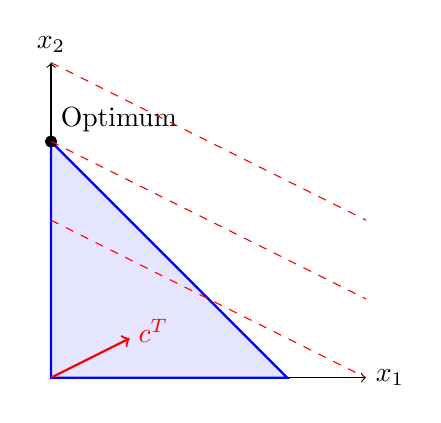
\begin{tikzpicture}
\draw[->] (0,0) -- (4,0) node[right] {$x_1$};
\draw[->] (0,0) -- (0,4) node[above] {$x_2$};

% Constraints and feasible region
\fill[blue!10] (0,0) -- (0,3) -- (1,2) -- (3,0) -- cycle;
\draw[blue,thick] (0,0) -- (0,3) -- (1,2) -- (3,0) -- cycle;

% Objective function vector
\draw[->,red,thick] (0,0) -- (1,0.5);
\node[red] at (1.3,0.6) {$c^T$};

% Optimum point
\filldraw[black] (0,3) circle (2pt) node[above right] {Optimum};

% Objective function level lines
\draw[red,dashed] (0,4) -- (4,2);
\draw[red,dashed] (0,3) -- (4,1);
\draw[red,dashed] (0,2) -- (4,0);

\end{tikzpicture}
\caption{Feasible region and optimum point in linear programming}
\label{fig:linear_programming}
\end{marginfigure}

\subsubsection{Quadratic Programming}

Quadratic programming (QP) deals with optimization problems where the objective function is quadratic and the constraints are linear:

\begin{equation}
\begin{aligned}
\min & \quad \frac{1}{2}x^TQx + c^Tx \\
\text{s.t.} & \quad Ax = b \\
& \quad x \geq 0
\end{aligned}
\end{equation}

Here, $Q$ is a symmetric matrix. If $Q$ is positive (semi) definite, the problem is convex and finding the global optimum is relatively easy.

\paragraph{Solution Methods}
Various solution methods have been developed for quadratic programming problems:
\begin{itemize}
    \item \textbf{Active Set Methods:} Solves unconstrained optimization subproblems by making predictions about which constraints are active
    
    \item \textbf{Interior Point Methods:} Approaches the optimum point by passing through the interior of the feasible region
    
    \item \textbf{Sequential Quadratic Programming (SQP):} Solves nonlinear optimization problems by dividing them into quadratic subproblems
\end{itemize}

\begin{tcolorbox}[title=QP Applications in Structural Engineering]
\begin{itemize}
    \item \textbf{Elastic Deformation Minimization:} Using the structure's stiffness matrix to minimize deformation under specific loads
    
    \item \textbf{Dynamic Behavior Optimization:} Using the structure's mass and stiffness matrices to optimize dynamic response
    
    \item \textbf{Finite Element Model Calibration:} Minimizing the squares of differences between experimental and numerical data
    
    \item \textbf{Weight and Displacement Optimization:} Multi-objective optimization involving both weight and displacement energy
\end{itemize}
\end{tcolorbox}

\paragraph{Structural Compliance Minimization Example}
A common quadratic programming problem in structural design is the minimization of compliance (or deformation energy) under a volume constraint:

\begin{equation}
\begin{aligned}
\min & \quad \frac{1}{2}F^Tu \\
\text{s.t.} & \quad Ku = F \\
& \quad \sum_{e=1}^{n_e} v_e\rho_e \leq V \\
& \quad 0 \leq \rho_e \leq 1, \quad e = 1, \ldots, n_e
\end{aligned}
\end{equation}

Where:
\begin{itemize}
    \item $u$: displacement vector
    \item $F$: force vector
    \item $K$: global stiffness matrix
    \item $\rho_e$: material density for element $e$ (design variable)
    \item $v_e$: volume of element $e$
    \item $V$: allowed total volume
\end{itemize}

This formulation forms the basis of topology optimization and is the starting point of the SIMP (Solid Isotropic Material with Penalization) method.

\subsection{Modern Classical Optimization Algorithms}

Modern extensions of classical optimization methods aim to solve large and complex structural optimization problems using various approaches. In this section, we will discuss more advanced versions of classical methods.

\subsubsection{Secant Methods and Structural Applications}

Secant methods are approaches developed to eliminate the requirement of calculating the Hessian matrix in the Newton method. These methods create an approximate estimate of the Hessian matrix using gradient information.

The most common secant methods are:
\begin{itemize}
    \item \textbf{Broyden Method:} Used in solving general nonlinear equation systems
    \item \textbf{DFP (Davidon-Fletcher-Powell) Method:} One of the first examples of quasi-Newton methods
    \item \textbf{BFGS (Broyden-Fletcher-Goldfarb-Shanno) Method:} Has become standard in many fields including structural optimization
\end{itemize}

In the BFGS method, the approximate value of the Hessian matrix is updated as follows:
\begin{equation}
B_{k+1} = B_k - \frac{B_k s_k s_k^T B_k}{s_k^T B_k s_k} + \frac{y_k y_k^T}{y_k^T s_k}
\end{equation}

Where:
\begin{itemize}
    \item $s_k = x_{k+1} - x_k$
    \item $y_k = \nabla f(x_{k+1}) - \nabla f(x_k)$
\end{itemize}

The BFGS method is widely used in structural optimization problems, especially when there are many design variables.

\paragraph{Advantages of BFGS in Structural Optimization}
\begin{itemize}
    \item \textbf{Memory Efficiency:} Applicable even to large-scale problems with the L-BFGS variant
    \item \textbf{Superlinear Convergence:} Convergence rate increases as it approaches the optimum point
    \item \textbf{Numerical Stability:} More stable than the Newton method
    \item \textbf{Integration with Line Search:} Can be combined with strong line search strategies
\end{itemize}

\subsubsection{Trust Region and Line Search Strategies}

The performance of gradient-based optimization methods depends largely on step size selection. Line search and trust region are two fundamental strategies developed for determining step size.

\paragraph{Line Search Strategies}
In line search methods, after determining the search direction $d_k$, a suitable step size $\alpha_k$ is found:
\begin{equation}
x_{k+1} = x_k + \alpha_k d_k
\end{equation}

Various criteria are used to determine the optimal step size:
\begin{itemize}
    \item \textbf{Armijo Condition:} Guarantees that the step size provides sufficient decrease in the function value
    \item \textbf{Wolfe Conditions:} In addition to the Armijo condition, requires that the gradient change satisfies a certain ratio
    \item \textbf{Goldstein Conditions:} Ensures both decrease in function value and that the step size is not too small
\end{itemize}

\paragraph{Trust Region Approach}
In trust region methods, a region where the model is reliable is defined and the model is minimized within this region:
\begin{equation}
\begin{aligned}
\min & \quad m_k(p) = f_k + g_k^Tp + \frac{1}{2}p^TB_kp \\
\text{s.t.} & \quad \|p\| \leq \Delta_k
\end{aligned}
\end{equation}

Where:
\begin{itemize}
    \item $m_k(p)$: quadratic model of the function at the $k$th iteration
    \item $f_k = f(x_k)$, $g_k = \nabla f(x_k)$
    \item $B_k$: Hessian matrix or its approximation
    \item $\Delta_k$: trust region radius
\end{itemize}

In each iteration, the trust region radius is updated by comparing the model prediction with the actual function change.

\begin{tcolorbox}[title=Trust Region Applications in Structural Engineering]
The trust region approach is particularly preferred in structural engineering in the following cases:
\begin{itemize}
    \item \textbf{Ill-Conditioned Problems:} When the condition number of the stiffness matrix is high
    
    \item \textbf{Nonlinear Behavior:} In structural analyses involving material or geometric nonlinearity
    
    \item \textbf{Unstable Systems:} In problems close to instability points such as buckling analysis
    
    \item \textbf{Multi-physics Analyses:} In complex multi-physics problems such as thermal-structural, fluid-structure interaction
\end{itemize}
\end{tcolorbox}

\subsubsection{Sequential Constraint Programming}

Sequential Constraint Programming (SCP) is an effective approach developed for solving structural optimization problems. This method solves the nonlinear problem by transforming it into a series of linear subproblems.

The basic approach of SCP:
\begin{itemize}
    \item Linearizes nonlinear constraints around the current iteration point
    \item Solves the linearized problem
    \item Uses the solution as a new iteration point
    \item Repeats until convergence
\end{itemize}

This method, with its more advanced variants such as MMA (Method of Moving Asymptotes), is widely used in structural topology optimization.

The main advantages of MMA in structural optimization:
\begin{itemize}
    \item Efficiency in large-scale topology optimization problems
    \item Effective handling of nonlinear constraints
    \item Stable convergence by reducing oscillations
    \item Suitability for parallel computing
\end{itemize}

\begin{figure}
\centering
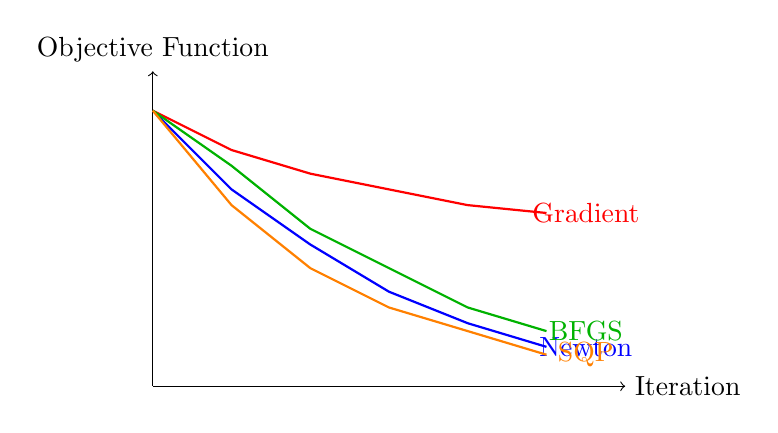
\begin{tikzpicture}
\draw[->] (0,0) -- (6,0) node[right] {Iteration};
\draw[->] (0,0) -- (0,4) node[above] {Objective Function};

% Gradient descent
\draw[red,thick] plot coordinates {(0,3.5) (1,3.0) (2,2.7) (3,2.5) (4,2.3) (5,2.2)};
\node[red] at (5.5,2.2) {Gradient};

% Newton
\draw[blue,thick] plot coordinates {(0,3.5) (1,2.5) (2,1.8) (3,1.2) (4,0.8) (5,0.5)};
\node[blue] at (5.5,0.5) {Newton};

% BFGS
\draw[green!70!black,thick] plot coordinates {(0,3.5) (1,2.8) (2,2.0) (3,1.5) (4,1.0) (5,0.7)};
\node[green!70!black] at (5.5,0.7) {BFGS};

% SQP
\draw[orange,thick] plot coordinates {(0,3.5) (1,2.3) (2,1.5) (3,1.0) (4,0.7) (5,0.4)};
\node[orange] at (5.5,0.4) {SQP};

\end{tikzpicture}
\caption{Comparison of convergence behaviors of different optimization algorithms}
\label{fig:convergence_comparison}
\end{figure}

\subsection{Conclusion and Transition to Modern Methods}

Classical optimization methods still hold great importance in solving various problems encountered in structural engineering. These methods form the foundation of modern meta-heuristic algorithms and artificial intelligence-based approaches.

\begin{tcolorbox}[title=Comparison of Classical and Modern Methods]
\begin{itemize}
    \item \textbf{Classical Methods:} Mathematical robustness, exact convergence guarantees, efficiency
    \item \textbf{Modern Methods:} Global search for multi-modal functions, parallel computing, flexibility in handling complex constraints
\end{itemize}
\end{tcolorbox}

Today, hybrid methods that combine the strengths of classical algorithms with the flexibility of modern approaches are receiving great interest. These hybrid approaches provide effective solutions, especially in large-scale and multi-objective structural optimization problems.
